\section{Unity 3D} % (fold)
\label{sec:unity_3d}

\subsection{O Unity }
\label{sub:o_unity}
	A unidade é um IDE de desenvolvimento de jogos com um potente mecanismo de renderização e totalmente integrado com um conjunto de ferramentas que permitem criação de conteúdos interativos em varias plataformas e em  3d ou 2d.Além disso é possivel gerar builds para de 16 plataformas  como o linux , android ,windows e iOS com um alto nivel de qualidade pois é possível utilizar recursos prontos da Assert Store e de comunidades de compartilhamento de conhecimentos. 
	Para esse projeto foi escolhido o Unity pois  além dos benefícios citados acima com ele é possível que o desenvolvimento seja mais agil, em menos tempo e com umcusto menor e com uma qualidade razoável. 

\subsection{Workflow} % (fold)
\label{sub:workflow}
	Com o intuito de simplificar o processo de criação e produção de software, o Unity oferece um ambiente de trabalho com diversas ferramentas integradas para o desenvolvimento para a possibilitar a criação de mundos complexos com bloco de construção de cenas rapidamente escaláveis, implementar fluxos de controle utilizando linguagens altamente utilizadas no mercado como C\# e Java Script, com uma perfomace de tempo de compilação. Além disso durante o processo de criação é possível economizar tempo utilizando elementos prontos, salas e forúm de bate papo para distribuição de conhecimentos e resolução de problemas e dúvidas.

\begin{figure}[h]
  \centering
  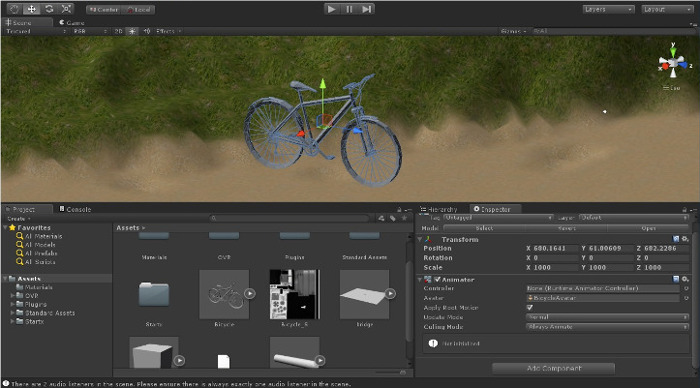
\includegraphics[width=0.8\textwidth]
      {figuras/bike.png}
  \caption{Edição de objeto no Unity}
  \label{coordenadas-rift}
\end{figure}

\subsection{Modelagem de Elementos} % (fold)
\label{sub:modelagem}
	Para a utilização de elementos no Unity é necessario a criação de objetos 3d, para isso pode ser utilizado qualquer um das IDE mais utilizadas do mercado tais como Maya , 3DMax, Blender ,Cinema4D, Modo, Lightwave, Cheetah3D, entre outros. A manipulação e ajustes de objetos em 3D está sendo realizada através da utilização da ferramenta blender  que é uma plataforma livre de alto desempenho que permite além da modelagem para a criação de objetos 3D e contém ferramentas para animações, criação de jogos, construção de foto realismo, simulações de fluidos, edição de vídeos,entre outros.Depois de feito os ajustes nos modelos o Blender possui suporte para exportar objetos nos formatos de arquivo: 3DS,DXF,FBX,OBJ,LWO,SVG,STL entre outros.

\begin{figure}[h]
  \centering
  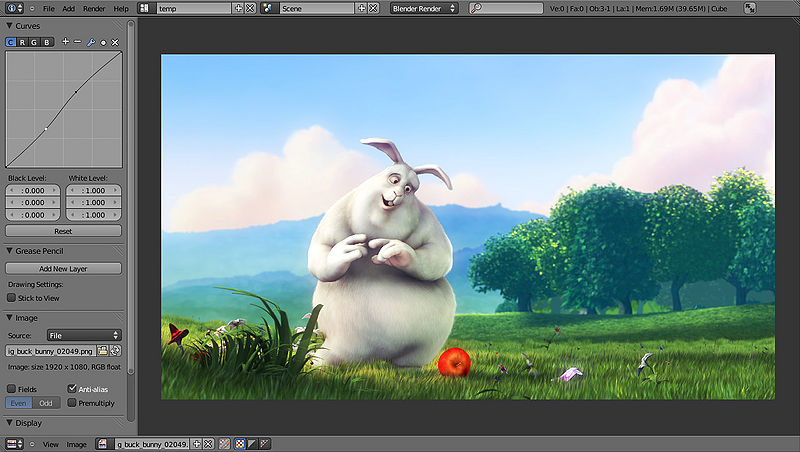
\includegraphics[width=0.8\textwidth]
      {figuras/blender.png}
  \caption{Renderização de \textit{Bick Buck Bunny} sendo feita no Blender}
  \label{coordenadas-rift}
\end{figure}

\subsection{SDK OculusVR}
\label{sub:sdk_ovr}
      Nos primeiros passos para a integração do Oculus Rift com o Unity foi necessário a utilização de uma SDK\footnote{ SDK encontrada em \url{https://developer.oculusvr.com/?action=dl&v=8 }} do próprio Oculus Rift ,que atualmente possui as versões 0.2, 0.3 e 0.4, que permite extrair dados do oculus e manipulos utilizando C++. No entanto como o Unity possui suporte para o plugin do Oculus Rift, que são scripts oriundos da SDK que ao invés de ser implementada em C++ é implementada em C\#, foi adotado o mesmo para auxiliar no controle do ambiente virtual no Unity.

\subsection{Criação de Scripts}
\label{sub:criacao_de_scripts}






